\documentclass[11pt, oneside]{article}   	% use "amsart" instead of "article" for AMSLaTeX format
\usepackage{geometry}                		% See geometry.pdf to learn the layout options. There are lots.
\geometry{letterpaper}                   		% ... or a4paper or a5paper or ... 
%\geometry{landscape}                		% Activate for for rotated page geometry
%\usepackage[parfill]{parskip}    		% Activate to begin paragraphs with an empty line rather than an indent
\usepackage{graphicx}				% Use pdf, png, jpg, or eps� with pdflatex; use eps in DVI mode
								% TeX will automatically convert eps --> pdf in pdflatex		
\usepackage{amssymb}
\usepackage{amsmath}
\usepackage{csvsimple}
\usepackage{dsfont}
\usepackage{listings}
%\usepackage[framed,numbered,autolinebreaks,useliterate]{mcode}  % mcode.sty Needs To Be in .tex directory!!
\usepackage{csvsimple}
%\usepackage[cm]{fullpage}

\title{FINC 520: Time Series \\
	Problem Set \#4}
\author{Qiushi Huang \\
	   Marius Ring }
	   
	   
\begin{document}
\maketitle
%\date{}							% Activate to display a given date or no date

\section{Question 1}

\subsection{part (a)}

We can rewrite the GARCH(1,1) as

\begin{align} \epsilon_t^2 = \omega + (\alpha+\beta) \epsilon_{t-1}^2 - \beta v_{t-1} + v_t \end{align}
\begin{align} v_t =  \epsilon_t^2-\sigma_t^2 = (z_t^2-1)\sigma_2^2 \end{align}
\begin{align} z_t \ \sim \mathrm{I.I.D.} \ \mathrm{N}(0,1) \end{align}

We find that
\begin{align} \mu \equiv \mathbb{E}\epsilon_t^2=\frac{\omega}{1-\alpha-\beta} \end{align}

Thus we may write
\begin{align} \epsilon_t^2 -\mu = (\alpha+\beta)( \epsilon_{t-1}^2 -\mu) - \beta v_{t-1} + v_t \end{align}


Then we use the Yule-Walker (not White-Walker as in Game of Thrones!!) method to find the autocorrelations for $\epsilon_t^2$, which will be the same as those of $y_t^2$ under our assumption.

The first autocorrelation:
\begin{align} \rho_1= \frac{\alpha(1-\alpha\beta-\beta^2)}{1-2\alpha\beta-\beta^2} \end{align}

Which provides us with all the subsequent ones due to p=q=1 in the GARCH(p,q):
\begin{align} \rho_k= (\alpha+\beta)^{k-1}\rho_1 \end{align}

\subsection{ part(b)}

The heteroskedasticity consistent estimator for the asymptotic covariance matrix is 
\begin{align} \hat V = \hat Q^{-1} \Omega \hat Q^{-1} \end{align}

where
\begin{align} \hat \Omega = \frac{1}{T} \sum \hat \epsilon_t^2 y_{t-1}^2 \end{align}
\begin{align} \hat Q= \ \frac{1}{T} \sum y_{t-1}^2 \end{align}

We will have that 
\begin{align} \sqrt{T}(\hat \phi - \phi) \rightarrow  N(0,Q^{-1}\Omega Q^{-1}) \mathrm{ \ in \ distribution.}\end{align}

Where we can, asymptotically, replace $Q^{-1}\Omega Q^{-1}$ with $\hat V$.

\begin{align} \Omega = \mathrm{plim} \frac{1}{T} \sum \hat \epsilon_t^2 y_{t-1}^2 = \mathbb{E}\epsilon_t^2 \epsilon_{t-1}^2 = \rho_1 \gamma_0 +\mu^2 \end{align}
\begin{align} Q= \mathrm{plim}\frac{1}{T} \sum y_{t-1}^2 = \mathbb{E}\epsilon_{t-1}^2=\mu \end{align}

\begin{align} V= \frac{\rho_1\gamma_0+\mu^2}{\mu^2} \end{align}

where

\begin{align} \gamma_0 = 3\omega^2(1+\alpha+\beta)[(1-\alpha-\beta)(1-\beta^2-2\alpha\beta-3\alpha^2)]^{-1} \end{align}
\begin{align} \mu =\frac{\omega}{1-\alpha-\beta} \end{align}
\begin{align} \rho_1= \frac{\alpha(1-\alpha\beta-\beta^2)}{1-2\alpha\beta-\beta^2} \end{align}

So in the case where $\alpha=\beta=0$ we have that $\rho_1 \rightarrow 0$ and $V \rightarrow 1$.

Otherwise, it follows from the terms, and our assumptions on $\omega, \alpha,$ and $\beta$ that $\rho_1>0$, and thus 
\begin{align} V>1 \end{align}

\subsection{ part (c)}

 \centerline{ \csvautotabular{Matlab/PS4Q1c.csv} }
 
 \begin{align} \hat \phi_T = \left(\sum_{t=2}^T y_{t-1}^2 \right)^{-1} \sum_{t=2}^T y_t y_{t-1} \end{align}
 
 The asymptotic variance of  $\sqrt{T} \hat \phi_T$ will just be 1 under our $H_0$, and the assumption that error terms are IID Normal. We see this in part (d): just let $\rho_1=0$.
 \begin{align} 		\end{align}
 
 In A and B $V=1$ and the IID Normal assumptions on the error term hold, so we would expect to see that that we reject 5\% of the time, which we also do.
 
 IN C and D $V>1$, thus using the IID Normal assumption on the error term, we would be using a variance that is too low, and thus use a test statistic that is too high, and thus reject too often. i.e. \textbf{heteroskedasticity that is unaccounted for increases the size of the test beyond our confidence level.}
 
 
 
 \subsection{ part (d) information criterions }
 The 'approximate' log likelihood function for the AR(p) estimation, assuming that the error terms are IID, is this:
 \begin{align} logL=-\frac{T-p-1}{2}\log(2\pi)-\frac{T-p-1}{2}\log(\sigma^2)-\frac{1}{2} \sum_{t=p+1}^T \frac{\epsilon_t^2}{\sigma^2}
\end{align}
 \begin{align} \epsilon_t = y_t - \sum_{j=1}^p \phi_j y_{t-j} \end{align}
 
 \begin{align} \hat \sigma_p^2 = \frac{1}{T-p-1} \sum_{t=p+1}^T  \hat \epsilon_t^2 =\frac{1}{T-p-1} \sum_{t=p+1}^T\left( y_t - \sum_{j=1}^p \hat\phi_j y_{t-j} \right)^2 \end{align}
 
  Thus for our Information Criterion comparisons we use:
 \begin{align} \log \hat L_p = -\frac{T}{2}\log(\hat\sigma_p^2) \end{align}
 
 Since the first terms with $p$ in the logL above artificially increase the logL due to the nature of the conditional/approximate MLE. Also the third term depends only on $T$ and $p$ when we subsitute in for $\hat\sigma^2$
 
 The ICs are given by:
 
 \begin{align} BIC = -2 \log \hat L_p + p \log(T) = T\log\hat \sigma_p^2 + p \ log(T) \end{align}
 \begin{align} AIC= -2 \log \hat L_p + 2p = T\log\hat \sigma_p^2 + 2p \end{align}


 and $\hat \phi_T$ is our usual OLS estimate, regressing $y_t$ on $y_{t-1},...y_{t-p}$, with no intercept term.
 
 
 \subsubsection*{AIC results}
  \centerline{ \csvautotabular{Matlab/PS4Q1dAIC.csv} }
   \subsubsection*{BIC results}
  \centerline{ \csvautotabular{Matlab/PS4Q1dBIC.csv} }
  
  From theory we would expect that both AIC and BIC would in the limit never pick a $p$ that was too small, and in the limit BIC will also not pick a $p$ that is too big. We also expected $AIC$ to be 'less conservative', i.e., choosing a higher number of lags, and possibly not be consistent towards the true $p=0$.
  
  The simulation results are well aligned with theory. We see that AIC more often than BIC picks too large $p$. We also see as $T\rightarrow 1000$ that BIC is a lot more consistent towards the true $p=1$ than AIC for the setups $G$ and $H$.
  
  \newpage
 \section{Question 2}
 
 \subsection{(a) time series model, covariance stationarity, invertibility}
 
 \begin{align} y_t^h=\gamma_h(L)\epsilon_t \end{align}
 \begin{align} \gamma_h(L)=\sum_{j=0}^{h-1} L^j \end{align}
 
 So clearly $y_t^h$ is an MA(h-1) process. For h=1 it is just white noise. For h=0 it is not well defined. 
 
 Any MA process is covariance stationary.However, it is \textbf{not} invertible, since \textbf{all} the roots of $\gamma_h(Z)=0$, for any $h\ge2$, lie \textbf{on} the unit circle.
 
 \subsection{(b) Gain and The Phase}
 
 The Gain, $G(w)$, and the Phase, $\theta(w)$, are defined as parameters in the exponential form of $\gamma_h(e^{iw})$:
 
 \begin{align} \gamma_h(e^{iw})=G(w)e^{i\theta(w)} \end{align}
 
 We can write
 
 \begin{align} \gamma_h(e^{iw})= 1+\sum_{j=1}^{h-1}(e^{iw})^j \end{align}
 
 We know that the gain will be
 \begin{align} G_h(w) = \mid  \gamma_h(e^{iw}) \mid =\left \vert 1+\sum_{j=1}^{h-1}e^{ijw} \right \vert \end{align}
 
 We could write this out in terms of cosines and sines, but it's not very useful, especially not for deriving the phase:
 
 \begin{align} \theta_h(w) = \frac{1}{-i}\log \left(\frac{\gamma_h(e^{iw})}{G_h(w)} \right) \end{align}
 
 or more precisely
 \begin{eqnarray} \theta_h(w) &=& \frac{1}{-i}\log \left(\frac{1+\sum_{j=1}^{h-1}e^{ijw}}{ \left \vert 1+\sum_{j=1}^{h-1}e^{ijw} \right \vert} \right) \\
 	&=& \frac{1}{2i}\log \left(\frac{(1+\sum_{j=1}^{h-1}e^{ijw})^2}{ \left \vert 1+\sum_{j=1}^{h-1}e^{ijw} \right \vert^2} \right) \\
	&=& \frac{1}{2i}\log \left(\frac{(1+\sum_{j=1}^{h-1}e^{ijw})^2}{ \left ( 1+\sum_{j=1}^{h-1}e^{ijw} \right )\left ( 1+\sum_{j=1}^{h-1}e^{-ijw} \right )} \right) \\
	&=& \frac{1}{2i}\log \left(\frac{e^{i(h-1)w}}{e^{i(h-1)w}}\frac{1+\sum_{j=1}^{h-1}e^{ijw}}{\left ( 1+\sum_{j=1}^{h-1}e^{-ijw} \right )} \right) \\
	&=& \frac{1}{2i}\log \left(e^{i(h-1)w}\frac{1+\sum_{j=1}^{h-1}e^{ijw}}{\left ( 1+\sum_{j=1}^{h-1}e^{ijw} \right )} \right) \\
	&=& \frac{1}{2i}\log \left(e^{i(h-1)w}\right) \\
	&=& \frac{i(h-1)w}{2i} = \frac{h-1}{2}w \\\\
 \end{eqnarray}
 
 which will be a real-valued function, and well defined for $w\in [0,\frac{2\pi}{h-1}]$.

 The general phase looks like this, where it "resets" at every  $\frac{2\pi}{h-1}$th frequency. The below plot is for $h=3$.
 
 \centerline{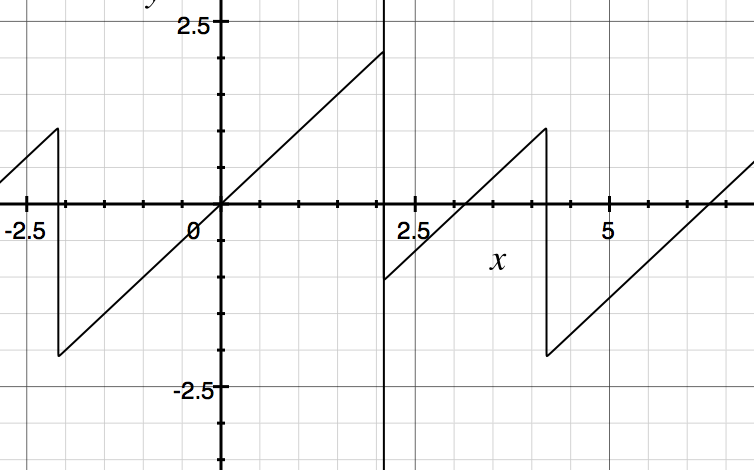
\includegraphics[scale=0.5]{phase.png}}
  
  
  \subsection{(c) Spectrum of $y_t,h$}
  
  We use the fact that this is just a filter of a white noise process with spectrum $\frac{\sigma_{\epsilon}^2}{2\pi}$, thus
  
  \begin{align} f_{y_{h}}(w) = \left \lvert 1 + \sum_{j=1}^{h-1} e^{-ijw} \right \rvert ^2 \frac{\sigma_{\epsilon}^2}{2\pi} \end{align}
  
  Again, complicating this by adding sines and cosines does not add any intuition. Instead we plot it for $h=2,3,4$, where the flattest one is h=2, and the waviest is h=4, and we set $\sigma_\epsilon^2=1$
  
   \centerline{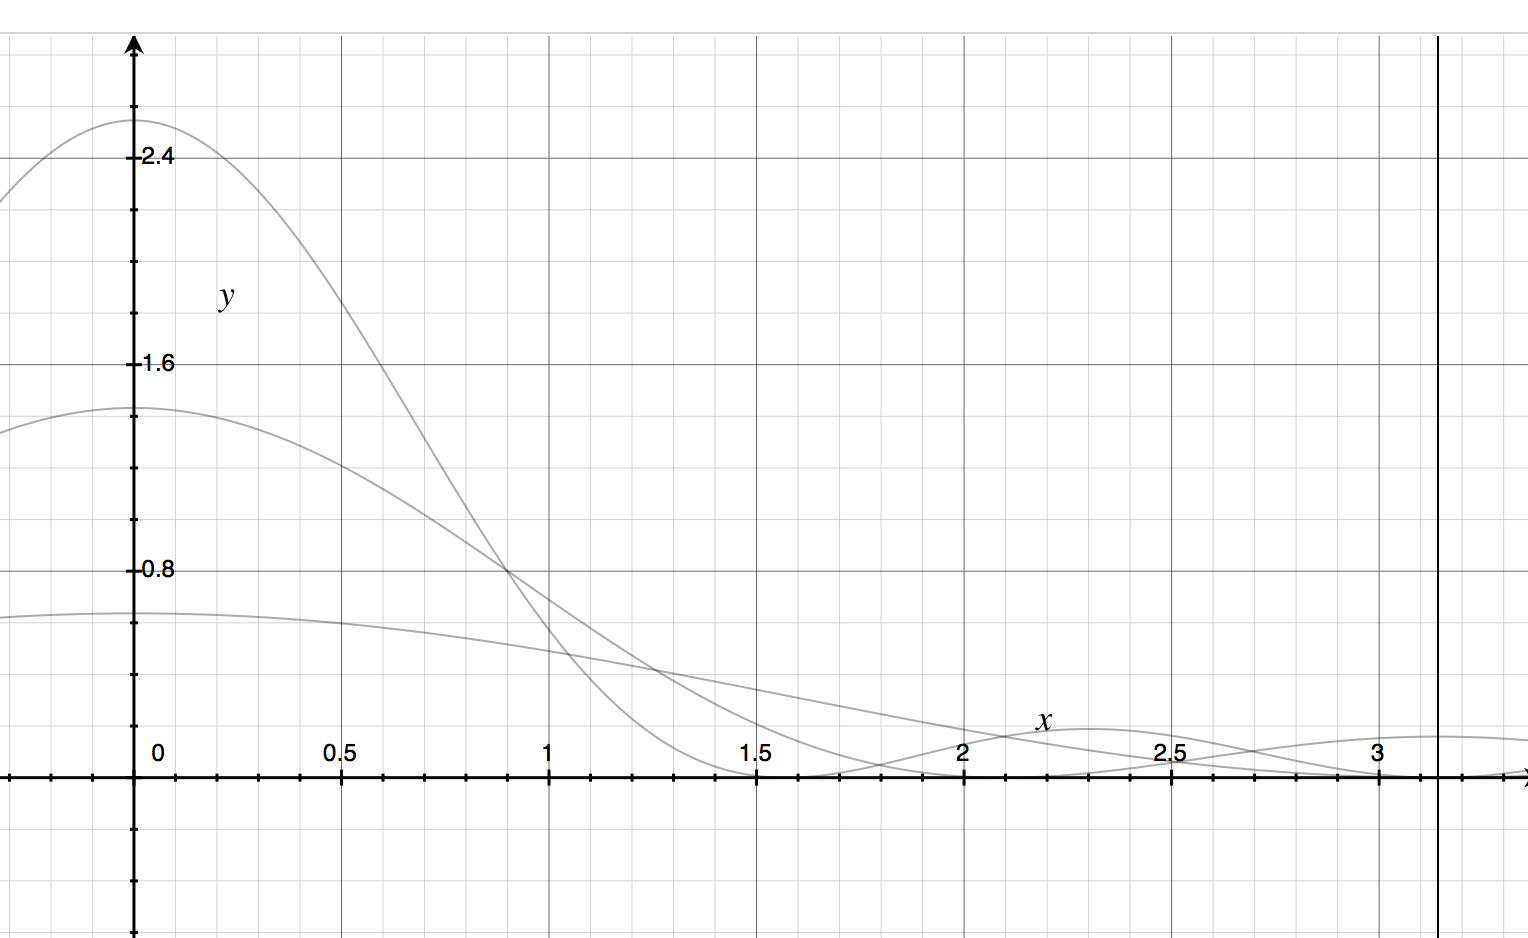
\includegraphics[scale=0.5]{spectrum.png}}
  
  
  
  
  
  \section{Question 3}
  
  \subsection{part (a) graph spectra}
  
  \begin{eqnarray}
  y_t &=&c_t + u_t \\
  c_t &=& 0.9c_{t-1} + \epsilon_t = ... = \sum_{j=0}^{\infty} 0.9^j \epsilon_{t-j} \\
  u_t &=& \eta_t - 0.8 \eta_{t-1}
  \end{eqnarray}
  
  since $c_t$ and $u_t$ are MA processes with independent errors (of eachother), the covariances of $y_t$ will be the sum of the respective covariances for $c_t$ and $u_t$, and thus the spectrum for $y$ is the sum of the spectra of $c$ and $u$.
  
  Since both $c$ and $u$ are filters of unit variance white noise processe, with spectra $\frac{1}{2\pi}$, we can write the spectra of $c$ and $u$ as functions of the spectrum of a unit variance white noise process.
  
  Using the general formula
   \begin{equation} f(w) = \left \lvert  \Psi(e^{-iw})	\right \rvert^2f_{WN}(w) \end{equation}
   
   We obtain
  \begin{eqnarray}
  f_u(w) &=& \left \lvert 1-0.8e^{-iw}	\right \rvert^2 \frac{1}{2\pi} \\
  f_c(w) &=& \left \lvert \frac{1}{1-0.9e^{-iw}}\right \rvert^2 \frac{1}{2\pi}
  \end{eqnarray}
  
  \centerline{ 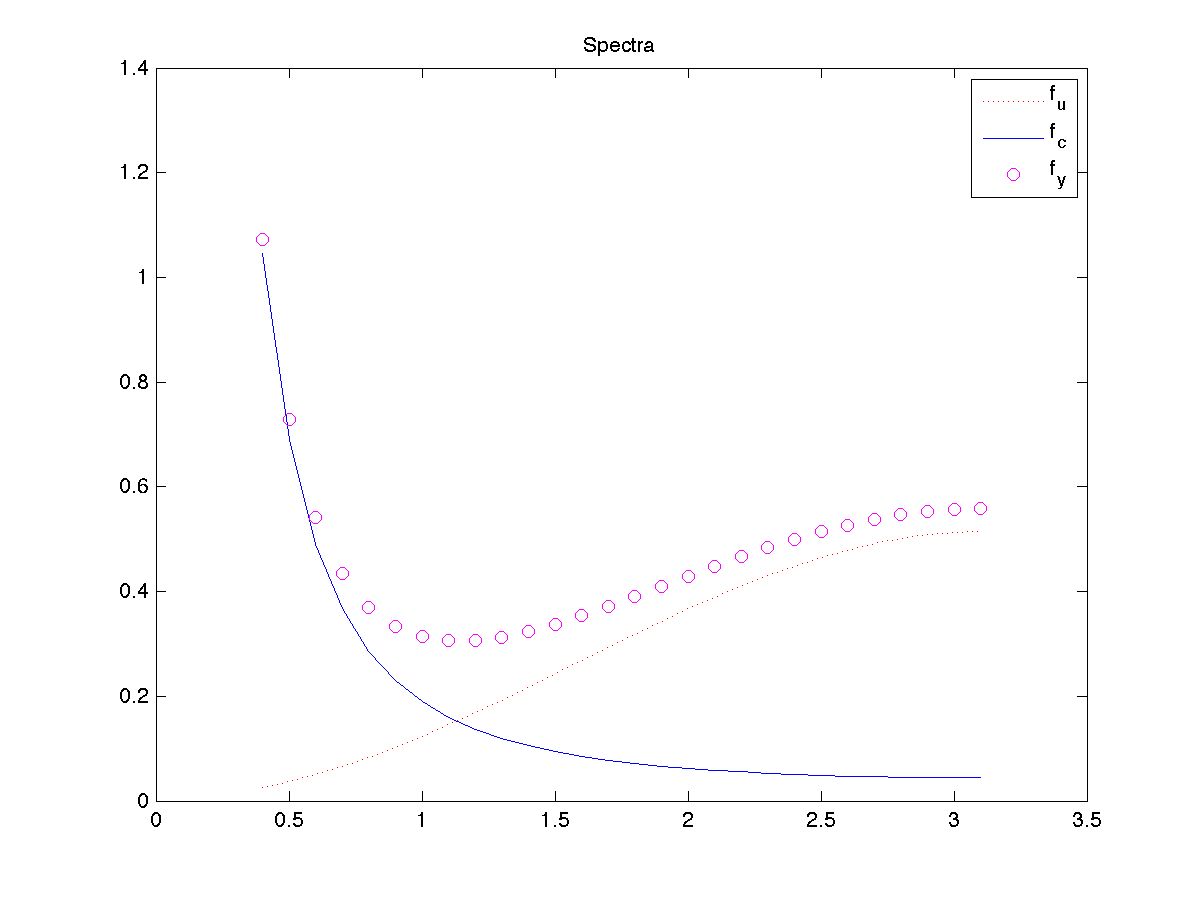
\includegraphics[scale=0.7]{Matlab/PS4Q3a.png}	}
  
  \subsection {b}
  Based on visual inspection, it seems that for $w<0.5$ the variance almost exclusively comes from $c_t$, while for $w>2$, the variance mostly comes from $u_t$. Thus an initial guess would be to create a filter $\delta(L)$ such that the spectrum of the filtered sequence looks like this, with $\underline{w}=1$.
  
  \begin{equation} f_{\hat c}(w) = \lvert \delta(e^{-iw}) \rvert^2 f_y(w)= \mathds{1}[w<\underline{w}]f_y(w) \end{equation}
  
  The first equality comes from the formula for how the spectrum of a filtered series depends on the raw series. The second equality is what we wish to achieve. Thus we must set:
  \begin{equation} \delta(e^{iw}) = \mathds{1}[w<\underline{w}] \end{equation}
  
Now we need to find 
\begin{equation} \delta(L)=\sum_{h=-\infty}^\infty \delta_h L^h \end{equation}

That satisfies
  \begin{equation} \delta(L)=\sum_{h=-\infty}^\infty \delta_h \delta(e^{iw})^h \end{equation}
  
  For this we use the Fourier Inversion Formula from class:
  \begin{equation} k(h): \sum_h \mid k(h) \mid < \infty \Rightarrow \left[ k(h)=\int_{-\pi}^{\pi} e^{ihw}r(w)dw \iff r(w)=\frac{1}{2\pi} \sum_h e^{-ihw}k(h) \right] \end{equation}
  
  \begin{equation} r(w) \equiv \delta(e^{-iw}), k(h)\equiv 2\pi \delta_h \Rightarrow \delta_h = \frac{1}{2\pi} \int_{-\pi}^{\pi} e^{ihw} \delta(e^{iw})dw \end{equation}
  \begin{equation} \Rightarrow  \delta(L) = \frac{1}{2\pi} \sum_{h=-\infty}^{\infty}  \left(\int_{-\pi}^{\pi} e^{ihw} \delta(e^{iw})dw \right) L^h \end{equation}
  \begin{equation} \Rightarrow  \delta(L) = \frac{1}{\pi} \sum_{h=-\infty}^{\infty}  \frac{\sin(h\underline{w})}{h\underline{w}} L^h \end{equation}
  
  But we need to cut it off at some point (L=50). So we use:
   \begin{equation} \Rightarrow  \delta(L) =  \sum_{h=-\infty}^{\infty} \mathds{1}[\lvert h\rvert \le50] \frac{\sin(h\underline{w})}{\pi h\underline{w}} L^h \end{equation}
  
    \begin{equation} \Rightarrow  \delta(L) =  \sum_{h=-50}^{50} \frac{\sin(h\underline{w})}{\pi h\underline{w}} L^h \end{equation}
  
  And since we choose $\underline{w}=1$:
  
      \begin{equation} \Rightarrow  \delta(L) =  \sum_{h=-50}^{50} \frac{\sin(h)}{\pi h} L^h \end{equation}
  For h=0, $\delta_0$=1.
  \subsection{(c)}
  Correlation: $0.9559$
  
  \centerline{ 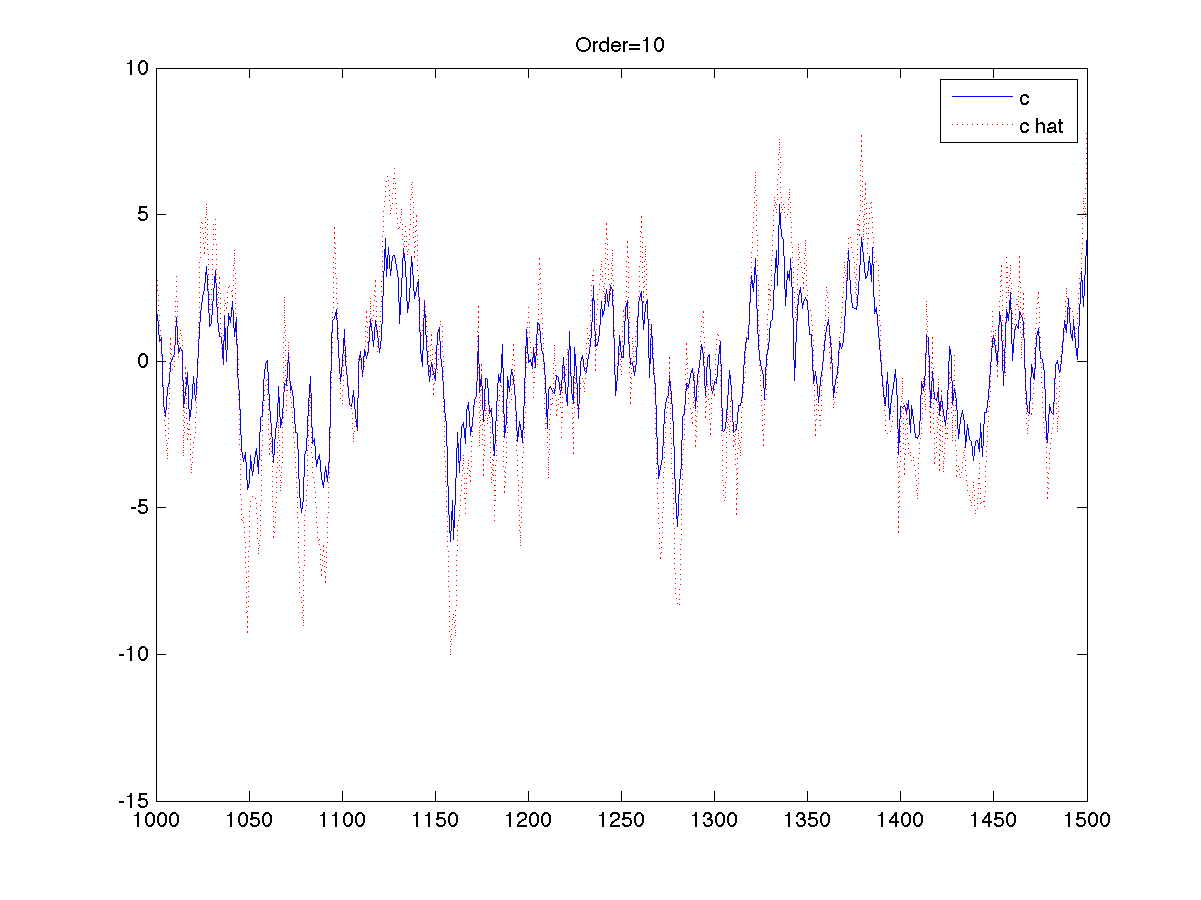
\includegraphics[scale=0.8]{Matlab/PS4Q3c.png} }
  
  \newpage
  
  \subsection{(d)}
  
  Correlation: $0.9561$ The correlation goes up. If we decrease the order further, the correlation goes up further. On one hand we are getting a poorer approximation to our filter, which we don't actually know is optimal, but on the other hand we are getting more data to use.
  
 \centerline{ 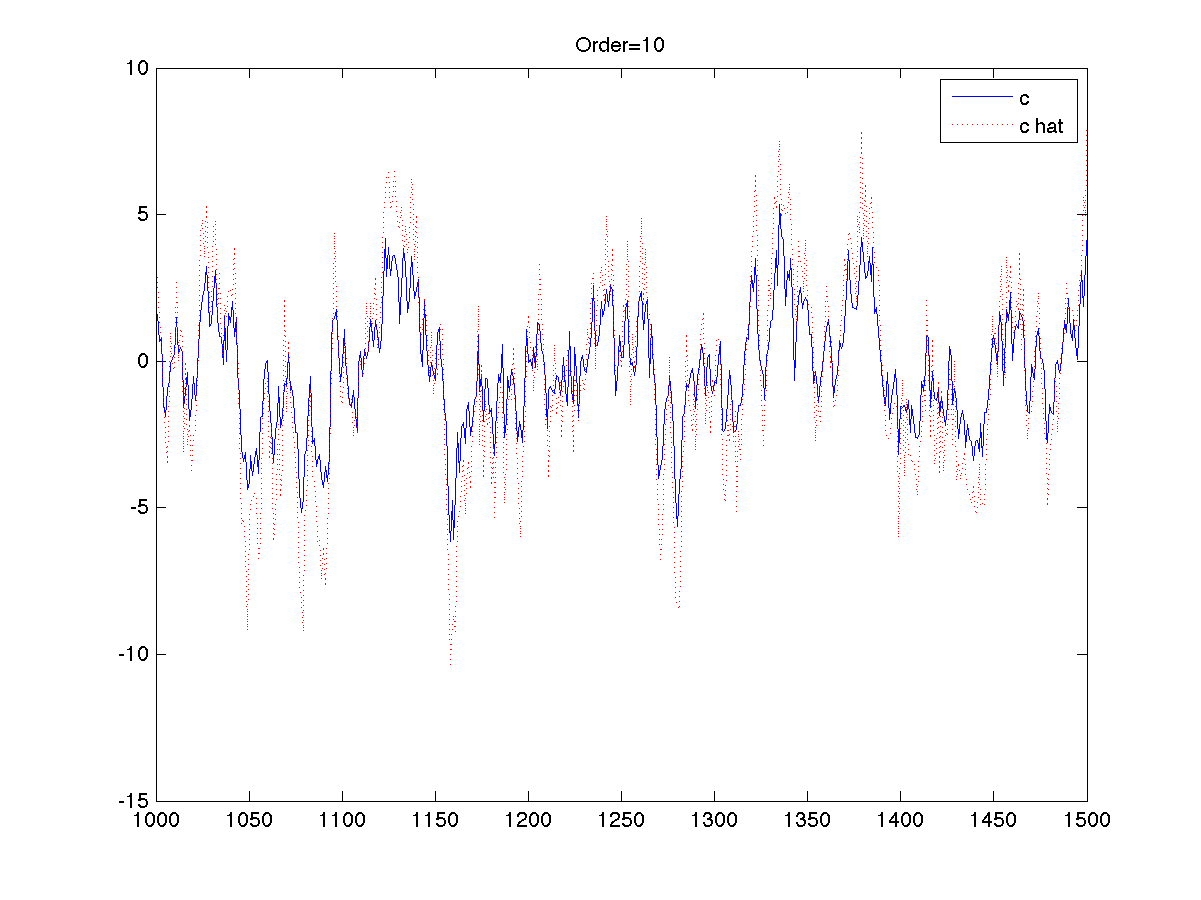
\includegraphics[scale=0.8]{Matlab/PS4Q3d.png} }
  
  
  
  
  
  
  
  
\end{document}  